\documentclass{sig-alternate}
%\documentclass{acm_proc_article-sp}

\makeatletter
\newif\if@restonecol

\let\algorithm\relax
\let\endalgorithm\relax
\usepackage[tight,footnotesize]{subfigure}
\usepackage {paralist}
\usepackage{comment}
\usepackage{array}
\usepackage{amsmath}
\usepackage{graphicx}
\usepackage{amssymb}
\usepackage{cite}
\usepackage{url}
\makeatother
\makeatletter
\providecommand{\tabularnewline}{\\}


\newtheorem{clm}{Claim}
\begin{document}

\title{STM Concurrency Control for Multicore Embedded Real-Time Software: Time Bounds and Tradeoffs%\thanks{\footnotesize{Approved for Public Release. Unlimited Distribution.}}
}


\author{
\alignauthor Mohammed El-Shambakey\\
\affaddr{ECE Dept., Virginia Tech}\\
\affaddr{Blacksburg, VA 24060}\\
\affaddr{USA}\\
\email{shambake@vt.edu}
\alignauthor Binoy Ravindran\\
\affaddr{ECE Dept., Virginia Tech}\\
\affaddr{Blacksburg, VA 24060}\\
\affaddr{USA}\\
\email{binoy@vt.edu}
}

\maketitle

\begin{abstract}
We consider software transactional memory (STM) concurrency control in multicore embedded real-time software. We investigate real-time contention managers (CMs) for resolving transactional conflicts, including those based on dynamic and fixed priorities, and establish upper bounds on transactional retries and task response times. We identify the conditions under which STM (with the proposed CMs) is superior to retry-loop lock-free synchronization. Presented work is analytical, so our results. Experimental evaluation will be done in future work.

\end{abstract}

\section{Introduction}
\label{sec:intro}

Embedded systems sense physical processes and control their behavior, typically through feedback loops. Since physical processes are concurrent, computations that control them must also be concurrent, enabling them to process multiple streams of sensor input and control multiple actuators, all concurrently. Often, such computations need to concurrently read/write shared data objects. Typically, they must also process sensor input and react in a timely manner. 

The de facto standard for programming concurrency is the threads abstraction, and the de facto synchronization abstraction is locks. 
Lock-based concurrency control has significant programmability, scalability, and compositionality challenges~\cite{Herlihy:2006:AMP:1146381.1146382}. Transactional memory (TM) is an alternative synchronization model for shared in-memory data objects that promises to alleviate these difficulties.  With TM, programmers write concurrent code using threads, but organize code that read/write shared objects as transactions, which appear to execute atomically. Two transactions conflict if they access the same object and one access is a write. When that happens, a contention manager (or CM)~\cite{Guerraoui:2005:TTT:1073814.1073863} resolves the conflict by aborting one and allowing the other to proceed to commit, yielding (the illusion of) atomicity. Aborted transactions are re-started, often immediately.  In addition to a simple programming model, TM provides performance comparable or superior to highly concurrent fine-grained locking and lock-free approaches~\cite{Saha:2006:MHP:1122971.1123001}, and is composable~\cite{Harris:2005:CMT:1065944.1065952}. Multiprocessor TM has been proposed in hardware, called HTM (e.g.,~\cite{austenmc:tcc:dissertation:2009}), and in software, called STM (e.g.,~\cite{sha95}), with the usual tradeoffs: HTM provides strong atomicity~\cite{austenmc:tcc:dissertation:2009}, has lesser overhead, but needs transactional support in hardware; STM is available on any hardware.


Given STM's programmability, scalability, and compositionality advantages, we consider it for concurrency control in multicore embedded real-time software. Doing so will require bounding transactional  retries, as real-time threads, which subsume transactions, must satisfy time constraints.  Retry bounds in STM are dependent on the CM policy at hand (analogous to the way thread response time bounds are scheduler-dependent). Thus, real-time CM is logical.

Designing a real-time CM is straightforward. Transactional contention can be resolved using dynamic or fixed priorities of parent threads, resulting in Earliest-Deadline-First (EDF) CM or Rate Monotonic Assignment (RMA)-based CM, respectively. But what upper bounds exist for transactional retries and thread response times under such CMs and respective multicore real-time schedulers, global EDF (G-EDF) and global RMA (G-RMA)? As lock-free protocols and STM do not use locks, how do they compare to each other? i.e., are there upper or lower bounds for transaction lengths below or above which is STM superior to lock-free?

We answer these questions. We consider EDF and RMA CMs, and establish their retry and response time upper bounds, and the conditions under which they outperform lock-free protocols. Our work reveals a key result: for most cases, for G-EDF/EDF CM and G-RMA/RMA CM to be better or as good as lock-free, the atomic section length under STM must not exceed half of the lock-free retry loop-length. However, in some cases, for G-EDF/EDF CM, the atomic section length can reach the lock-free retry loop-length, and for G-RMA/RMA CM, it can even be larger than the lock-free retry loop-length.  This means that, STM is more advantageous with G-RMA than with G-EDF.
These results, among others, for the first time, provide a
fundamental understanding of when to use, and not use, STM concurrency
control in multicore embedded real-time software, and constitute the
paper's contribution. 

We overview past and related efforts in Section~\ref{sec:past}. Section~\ref{sec:model} outlines the work's preliminaries. Sections~\ref{sec:g-edf-edf-cm} and~\ref{sec:g-rma-rma-cm}
establish response time bounds under G-EDF/EDF CM and G-RMA/RMA CM, 
respectively. We compare STM against lock-free approaches in Section~\ref{sec:comparison}. We conclude in Section~\ref{sec:conclusions}.
\section*{}
\section{Related Work}
\label{sec:past}

Transactional-like concurrency control without using locks, for real-time systems, has been previously studied in the context of non-blocking data structures (e.g.,~\cite{anderson95realtime}). Despite their numerous advantages over locks 
(e.g., deadlock-freedom), 
their programmability has remained a challenge. 
Past studies show that they are best suited for simple data structures where their retry cost is competitive to the cost of lock-based synchronization~\cite{bc+08}.  In contrast, STM is semantically simpler~\cite{Herlihy:2006:AMP:1146381.1146382}, and is often the only viable lock-free solution for complex data structures (e.g., red/black tree)~\cite{key-1} and nested critical sections~\cite{Saha:2006:MHP:1122971.1123001}.
%(The relationship between lock-free and STM is similar to that between programmer-controlled memory management and garbage collection.)


STM concurrency control for real-time systems has been previously studied in~\cite{manson2006preemptible,fahmy2009bounding,sarni2009real,schoeberl2010rttm,key-1,barrosmanaging}.


\cite{manson2006preemptible} proposes a restricted version of STM for uniprocessors. Uniprocessors do not need contention management.

\cite{fahmy2009bounding} bounds response times in distributed multiprocessor systems with STM synchronization. They consider Pfair scheduling, limited to small atomic regions with fixed size, and limit transaction execution to span at most two quanta. In contrast, we allow atomic regions with  arbitrary duration. 

\cite{sarni2009real} presents real-time scheduling of transactions and serializes transactions based on deadlines. However, the work does not bound retries and response times, nor establishes  tradeoffs against lock-free approach. In contrast, we establish such bounds and tradeoffs.


\cite{schoeberl2010rttm} proposes real-time HTM, unlike real-time STM that we consider. 
The work does not describe how transactional conflicts are resolved. 
In contrast, we show how task response times can be met using different conflict resolution policies. 
Besides, the retry bound developed in~\cite{schoeberl2010rttm} assumes that the worst case conflict between atomic sections of different tasks occurs when the sections are released at the same time. However, we show that this is not the worst case. We develop retry and response time upper bounds based on much worse conditions.


The past work that is closest to ours is~\cite{key-1}, which upper bounds retries and response times for  EDF CM with G-EDF, and identify the tradeoffs against locking and lock-free protocols. Similar to~\cite{schoeberl2010rttm},~\cite{key-1} also assumes that the worst case conflict between atomic sections occurs when the sections are released simultaneously. 
In addition, we consider RMA CM, besides EDF CM.

The ideas in~\cite{key-1} are extended in~\cite{barrosmanaging}, which presents three real time CM designs. But no retry bounds nor schedulability analysis are presented for those CMs. 


\section{Preliminaries}
\label{sec:model}

We consider a multiprocessor system with $m$ identical processors and $n$ sporadic tasks $\tau_1, \tau_2,\ldots, \tau_n$. The $k^{th}$ instance (or job) of a task $\tau_i$ is denoted $\tau_i^k$. Each task $\tau_i$ is specified by its worst case execution time (WCET) $c_i$, its minimum period $T_i$ between any two consecutive instances, and its relative deadline $D_i$, where $D_i=T_i$. Job $\tau_i^j$ is released at time $r_i^j$ and must finish no later than its absolute deadline $d_i^j=r_i^j+D_i$. Under a fixed priority scheduler such as G-RMA, $p_i$ determines $\tau_i$'s (fixed) priority and it is constant for all instances of $\tau_i$. Under a dynamic priority scheduler such as G-EDF, a $\tau_i^j$'s priority, $p_i^j$, is determined by its absolute deadline. 
A task $\tau_j$ may interfere with task $\tau_i$ for a number of times during a duration $L$, and this number is denoted as $G_{ij}(L)$. 
$\tau_j$'s workload that interferes with $\tau_i$ during $L$ is denoted $W_{ij}(L)$.


\textit{Shared objects.} A task may need to access (i.e., read, write) shared, in-memory objects while it is executing any of its atomic sections, which are synchronized using STM. 
The set of atomic sections of task $\tau_i$ is denoted $s_i$. $s_i^k$ is the $k^{th}$ atomic section of $\tau_i$. 
Each object, $\theta$, can be accessed by multiple tasks. The set of objects accessed by $\tau_i$ is $\theta_i$ without repeating objects.
The set of atomic sections used by $\tau_i$ to access $\theta$ is $s_i(\theta)$, and the sum of the lengths of those atomic sections is $len(s_i(\theta))$. $s_i^k(\theta)$ is the $k^{th}$ atomic section of $\tau_i$ that accesses $\theta$. $s_i^k(\theta)$  executes for a duration $len(s_i^k(\theta))$.
% which is the whole length of the atomic section (and not just the part that accesses $\theta$). 
%Thus, for two objects $\theta_1$ and $\theta_2$ that are accessed within the same atomic section of $T_i$, $len(s_i^k(\theta1))=len(s_i^k(\theta2))$. 
If $\theta$ is shared by multiple tasks, then $s(\theta)$ is the set of atomic sections of all tasks accessing $\theta$, and the set of tasks sharing $\theta$ with $\tau_i$ is denoted $\gamma_i(\theta)$. Atomic sections are non-nested, and each atomic section is assumed to access only one object to enable comparison with retry-loop lock-free approach \cite{key-5} (if an atomic section is allowed to access more than one object, more complex lock-free approaches will be needed).

The maximum-length atomic section in $\tau_i$ that accesses $\theta$ is denoted $s_{i_{max}} (\theta)$, while the maximum one among all tasks is $s_{max} (\theta)$, and the maximum one among tasks with priorities lower than that of $\tau_i$ is $s_{max}^i (\theta)$.

\textit{STM retry cost.} If two or more atomic sections conflict, the CM will commit one section and abort and retry the others, increasing the time to execute the aborted sections. The increased time that an atomic section $s_i^p (\theta)$ will take to execute due to interference with another section $s_j^k (\theta)$, is denoted $W_{i}^{p}(s_{j}^{k}(\theta))$. 

The total time that a task $\tau_i$'s atomic sections have to retry is denoted $RC(\tau_i)$.
When this retry cost is calculated over the task period $T_i$ or an interval $L$, it is   denoted, respectively, as $RC(T_i)$ and $RC(L)$. 

\section{G-EDF/EDF CM Response Time}
\label{sec:g-edf-edf-cm}

Since only one atomic section among many that share the same object can commit at any time under STM, those atomic sections execute in sequential order.  A task $\tau_{i}$'s atomic sections are interfered by other tasks that share the same objects with $\tau_{i}$. An atomic section of $\tau_i$, $s_i^k(\theta)$, is aborted and retried by a conflicting atomic section of $\tau_j$, $s_j^l(\theta)$, if $d_j \le d_i$, by the EDF CM. We will use \emph{ECM} to refer to a multiprocessor system scheduled by G-EDF and resolves STM conflicts using the EDF CM. 



The maximum number of times a task $\tau_{j}$ interferes with $\tau_{i}$ is given in~\cite{key-2} and is shown in Figure~\ref{fig1}. 
Here, the deadline of an instance of $\tau_{j}$ coincides
with that of $\tau_{i}$, and $\tau_{j}^{1}$ is delayed by its maximum
jitter $J_{j}$, which causes all or part of $\tau_{j}^1$'s execution to overlap within $T_i$. From Figure~\ref{fig1}, it is seen that $\tau_{j}$'s maximum workload that interferes with $\tau_{i}$ (when there are no atomic sections) in $T_{i}$ is:
\begin{eqnarray}
W_{ij}\left(T_{i}\right) & \le & \left\lfloor\frac{T_{i}}{T_{j}}\right\rfloor c_{j}+min\left(c_{j},T_{i}-\left\lfloor\frac{T_{i}}{T_{j}}\right\rfloor T_{j}\right)\nonumber \\
 & \le & \left\lceil\frac{T_{i}}{T_{j}}\right\rceil c_{j}\label{eq11}\end{eqnarray}

For an interval $L<T_{i}$, the worst case pattern of interference is shown in Figure~\ref{fig2} where $\tau_{j}^{1}$ contributes by all its $c_j$ and $d_j^{k-1}$ does not have to coincide with $L$ as $\tau_j^{k-1}$ has a higher priority than that of $\tau_{i}$, and the workload of $\tau_{j}$ is:
\begin{equation}
W_{ij}\left(L\right)\le \left(\left\lceil\frac{L-c_{j}}{T_{j}}\right\rceil +1\right)c_{j}
\label{eq12}\end{equation}

Thus, the overall workload, over an interval $R$ is:
\begin{equation}
W_{ij}\left(R\right)=min\left(W_{ij}\left(R\right),W_{ij}\left(T_{i}\right)\right)\label{eq13}\end{equation}
where $W_{ij}(R)$ is calculated by~(\ref{eq12}) if $R<T_i$, otherwise, it is calculated by~(\ref{eq11}).

\begin{figure}%[htbp]
\centering
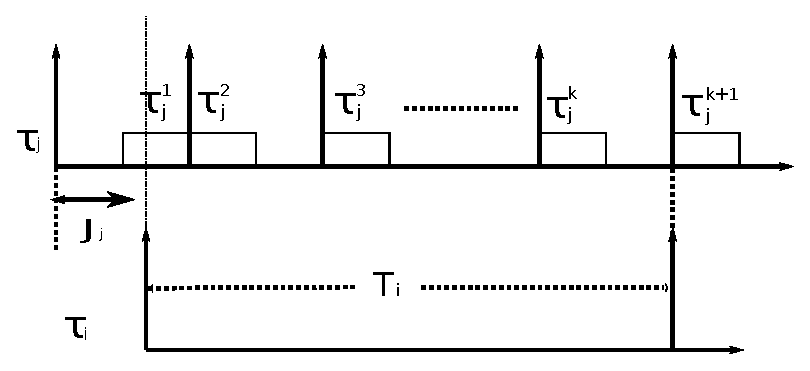
\includegraphics[bb=0bp 0bp 542bp 162bp,scale=0.5]{figures/figure9-a}
\caption{\label{fig1} Maximum interference between two tasks under G-EDF}
\end{figure}


\begin{figure}
\centering
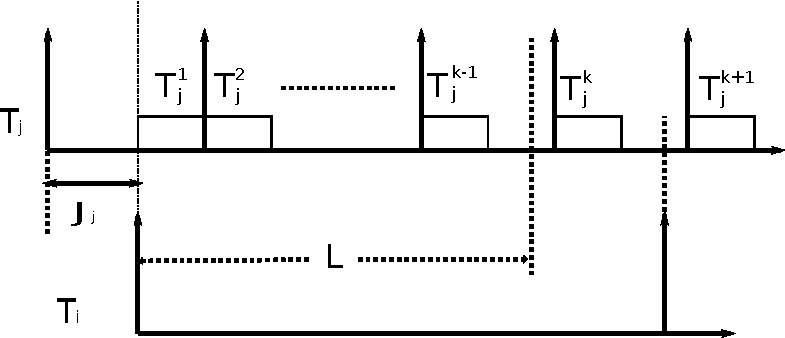
\includegraphics[bb=0bp 0bp 542bp 162bp,scale=0.5]{figures/figure9-b}
\caption{\label{fig2}Maximum interference during part $L$ of $T_{i}$}
\end{figure}



\subsection{Retry Cost of Atomic Sections}

\begin{figure*}
\centering
\subfigure[Early validation]{
            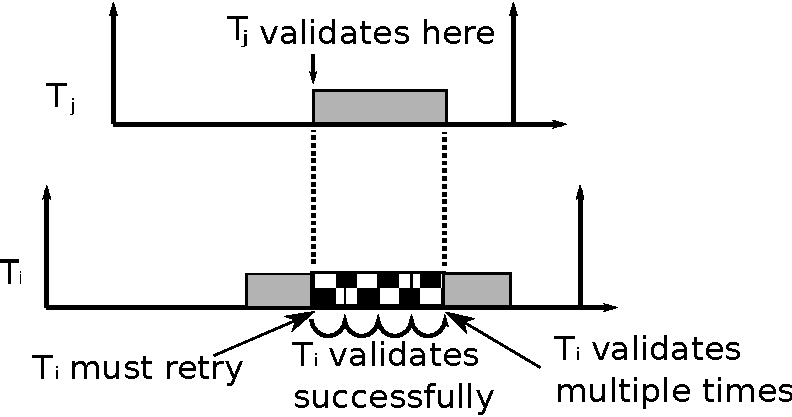
\includegraphics[scale=.45]{figures/figure5-a}
\label{fig5-a} 
}\hspace{1.2cm}
\subfigure[Lazy validation with $len(s_{i}^{k}(\theta))\le len(s_{j}^{l}(\theta))$]{
            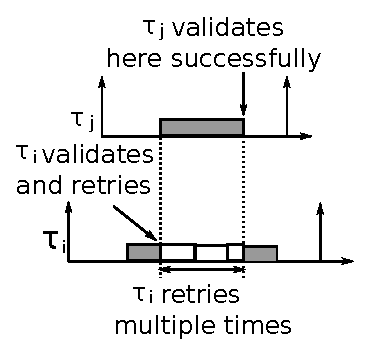
\includegraphics[scale=.65]{figures/figure5-b-1}
\label{fig5-b} 
}\hspace{1.5cm}
\subfigure[Lazy validation with $len(s_{i}^{k}(\theta))>len(s_{j}^{l}(\theta))$]{
            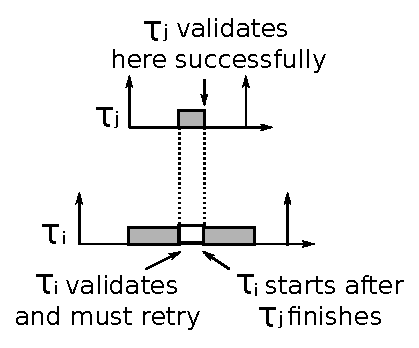
\includegraphics[scale=.65]{figures/figure5-c-1}
\label{fig5-c} 
}
\caption{Retry of $s_i^k(\theta)$ due to $s_j^l(\theta)$}  
\label{fig5}
\end{figure*}

\begin{clm}\label{gedf-edf}
Under ECM, a task $T_i$'s maximum retry cost during $T_i$ is upper bounded by:
\begin{eqnarray}
RC\left(T_{i}\right) & \le & \sum_{\theta\in\theta_{i}}\Bigg(\Big(\sum_{\tau_{j}\in\gamma(\theta)}\Big(\left\lceil\frac{T_{i}}{T_{j}}\right\rceil\sum_{\forall s_{j}^{l}(\theta)}len\big(s_{j}^{l}(\theta)\nonumber \\
 & + & s_{max}(\theta)\big)\Big)\Big)-s_{max}(\theta)+s_{i_{max}}(\theta)\Bigg)\label{eq3}\end{eqnarray}
\end{clm}
\begin{proof}
Given two instances $\tau_{i}^a$ and $\tau_{j}^b$, where $d_j^b \le d_i^a$. When a shared object conflict occurs, the EDF CM will commit the atomic section of $\tau_j^b$ while aborting and retrying that of $\tau_i^a$.
Thus, an atomic section of $\tau_i^a$, $s_{i}^{k}(\theta)$,
will experience its maximum delay when it is at its end of the atomic section, 
%%BR: You can say "...when it is at its end," CORRECT? Since you are referring to the same section. 
and the conflicting atomic section of $\tau_j^b$, $s_{j}^{l}(\theta)$, starts, because the whole $s_i^k (\theta)$ will be repeated after $s_j^l (\theta)$.

Validation (i.e., conflict detection) in STM is usually done in two ways~\cite{austenmc:tcc:dissertation:2009}: a) eager (pessimistic), in which conflicts are detected at access time, b) lazy (optimistic), in which conflicts are detected at commit time. Despite the validation time incurred (either eager or lazy),  
$s_{i}^{k}(\theta)$ will retry for the same time duration, which is $len(s_{j}^{l}(\theta)+s_i^k(\theta))$. Then, $s_i^k(\theta)$ can commit successfully  
unless interferred by another conflicting atomic section, as shown in Figure~\ref{fig5}. 

In Figure~\ref{fig5-a}, $s_{j}^{l}(\theta)$
validates at its beginning, due to early validation, and a conflict
is detected. So $\tau_{i}^a$ retries multiple times (because at the start of each retry, $\tau_{i}^a$ validates) 
during the execution of $s_{j}^{l}(\theta)$.
When $\tau_{j}^b$ finishes its atomic section, $\tau_{i}^a$ executes its atomic section. 

In Figure~\ref{fig5-b}, 
$\tau_{i}^a$ validates at its end (due to lazy validation), and detects a conflict with $\tau_{j}^b$.
Thus, it retries, and because its atomic section length is shorter
than that of $\tau_{j}^b$, it validates again within the execution
interval of $s_{j}^{l}(\theta)$. However, the EDF CM retries it again.
This process continues until $\tau_{j}^b$ finishes its atomic section.
If $\tau_{i}^a$'s atomic section length is longer than that of $\tau_{j}^b$,
$\tau_{i}^a$ would have incurred the same retry time, because
$\tau_{j}^b$ will validate when $\tau_{i}^a$ is retrying, and $\tau_{i}^a$ will
retry again, as shown in Figure~\ref{fig5-c}. Thus, the retry cost
of $s_{i}^{k}(\theta)$ is $len(s_{i}^{k}(\theta)+s_{j}^{l}(\theta))$.

If multiple tasks interfere with $\tau_{i}^a$ or
interfere with each other and $\tau_{i}^a$ (see the two interference examples in Figure~\ref{fig6}), then, in each case, each atomic section of the shorter deadline tasks contributes to the delay of $s_{i}^{p}(\theta)$ by its total length, plus a retry to some atomic section in the longer deadline tasks. For example,
$s_{j}^{l}(\theta)$ contributes by $len(s_{j}^{l}(\theta)+s_{i}^{p}(\theta))$
in both figures~\ref{fig6-a} and~\ref{fig6-b}. 
%%BR: YOu should say "..in both Figures~\ref{fig6-a} and~\ref{fig6-b}."
In Figure~\ref{fig6-b}, $s_{k}^{y}(\theta)$ causes a retry 
to $s_{j}^{l}(\theta)$, and $s_{h}^{w}(\theta)$ causes a retry to $s_{k}^{y}(\theta)$.


Since we do not know in advance which atomic section will be retried
due to another, we can safely assume that, each atomic section (that share the same object with  $\tau_i^a$) in a shorter deadline task contributes by its total length, in addition to the maximum length between all atomic sections that share the same object, $len(s_{max}(\theta))$. Thus, 
\begin{equation}
\mbox{\ensuremath{W_{i}^{p}\left(s_{j}^{k}\left(\theta\right)\right)\le len\left(s_{j}^{k}\left(\theta\right)+s_{max}\left(\theta\right)\right)}}\label{eq2}\end{equation}


Thus, the total contribution of all atomic sections of all other tasks
that share objects with a task $\tau_i$ 
to the retry cost of $\tau_i$ during $T_i$ is:
\begin{eqnarray}
RC\left(T_{i}\right) & \le & \sum_{\theta\in\theta_{i}}\sum_{\tau_{j}\in\gamma_i(\theta)}\Big(\left\lceil\frac{T_{i}}{T_{j}}\right\rceil\sum_{\forall s_{j}^{l}(\theta)}len\big(s_{j}^{l}(\theta)\nonumber \\
 & + & s_{max}(\theta)\big)\Big)\label{eq3-1}\end{eqnarray}



Here, $\left\lceil\frac{T_{i}}{T_{j}}\right\rceil\sum_{\forall s_{j}^{l}\left(\theta\right)}len\left(s_{j}^{l}\left(\theta\right)+s_{max}\left(\theta\right)\right)$ is  the contribution of all instances of $\tau_{j}$ during $T_{i}$. This contribution is added to all tasks. The last atomic section to execute is $s_{i}^{p}(\theta)$ ($\tau_i$'s atomic section that was delayed by conflicting atomic sections of other tasks). One of the other atomic sections (e.g., $s_{m}^{n}(\theta)$) should have a contribution $len(s_{m}^{n}(\theta)+s_{i_{max}}(\theta))$, instead of $len(s_{m}^{n}(\theta)+s_{max}(\theta))$. That is why one $s_{max}(\theta)$ should be subtracted, and $s_{i_{max}}(\theta)$ should be added (i.e., $s_{i_{max}}(\theta)-s_{max}(\theta)$). Claim follows.
\end{proof}

\begin{figure*}%[htbp]%
\centering%
\subfigure[Other atomic sections interfere only with $s_i^p(\theta)$]{
            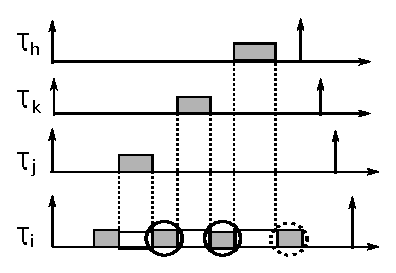
\includegraphics[scale=.65]{figures/figure6-a-1}
\label{fig6-a} 
}\hspace{1cm}
\subfigure[All atomic sections interfere with each other and $s_i^p(\theta)$]{
            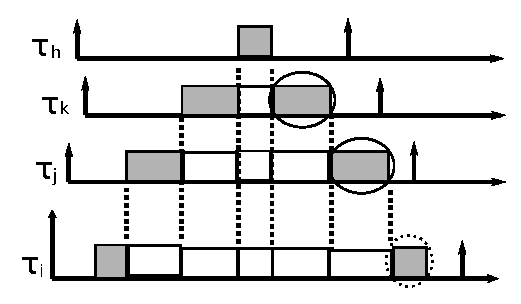
\includegraphics[scale=.6]{figures/figure6-b}
\label{fig6-b} 
}
\begin{tabular}{>{\centering}p{1cm}l}

\includegraphics[scale=0.45]{figures/circle} & Replaced in calculations by $s_{max}(\theta)$\tabularnewline

\includegraphics[scale=0.45]{figures/dotted_circle} & Replaced in calculations by $s_{i_{max}}(\theta)$\tabularnewline
\end{tabular}
\caption{Retry of $s_i^p(\theta)$ due to other atomic sections}  
\label{fig6}
\end{figure*}

\begin{clm}
Claim~\ref{gedf-edf}'s retry bound can be minimized as:
\begin{equation}
RC(T_{i})\le \sum_{\theta\in\theta_{i}}min(\Phi_1 , \Phi_2)\label{eq5}\end{equation}
where $\Phi_1$ is calculated by (\ref{eq3}) for one object $\theta$ (not the sum of $\theta \in \theta_i$),  and 
\begin{eqnarray}
\Phi_2 & = & \Bigg(\sum_{\tau_{j}\in\gamma_i(\theta)} \Big(\left\lceil\frac{T_{i}}{T_{j}}\right\rceil\sum_{\forall s_{j}^{l}(\theta)}len \big(s_{j}^{l}(\theta)\nonumber \\
 &  & +s_{max}^{*}(\theta) \big) \Big) \Bigg)-\bar{s}_{max}(\theta)+s_{i_{max}}(\theta)\label{eq4}\end{eqnarray}
 where $s^*_{max}$ is the maximum atomic section between all tasks, except $\tau_j$, accessing $\theta$. $\bar{s}_{max}(\theta)$ is the second maximum atomic section between all tasks accessing $\theta$.
\end{clm}
\begin{proof}
(\ref{eq3}) can be modified by noting that a task $\tau_j$'s atomic section 
may conflict with those of other tasks, but not with $\tau_j$. 
This is because, tasks are assumed to arrive sporadically, and  each instance finishes before the next begins. 
Thus, (\ref{eq2}) becomes:
\begin{equation}
W_i^p \left(s_j^k (\theta)\right)\le len\left(s_j^k (\theta)+s^*_{max}(\theta)\right)
\label{eq4-1}\end{equation}

To see why $\bar{s}{}_{max}(\theta)$ is used instead of $s_{max}(\theta)$, the maximum-length atomic section of each task that accesses $\theta$ is grouped into an array, in non-increasing order of their lengths. $s_{max}(\theta)$ will be the first element of this array, and $\bar{s}_{max}(\theta)$ will be the next element, as illustrated in Figure~\ref{fig7}, where the maximum atomic
section of each task that accesses $\theta$ is associated with
its corresponding task. According to (\ref{eq4-1}), all tasks
but $\tau_{j}$ will choose $s_{j_{max}}(\theta)$ as the value of $s_{max}^{*}(\theta)$.
But when $\tau_{j}$ is the one whose contribution is studied,
it will choose $s_{k_{max}}(\theta)$, as it is the maximum one not
associated with $\tau_{j}$. This way, it can be seen that the maximum
value always lies between the two values $s_{jmax}(\theta)$ and $s_{kmax}(\theta)$. 
Of course, these two values can be equal, or the maximum value can be associated with $\tau_i$ itself, and not with any one of the interfering tasks. In the latter case,
the chosen value will always be the one associated with $\tau_i$, which still lies between the two largest values. 

\begin{figure}[htbp]
\centering
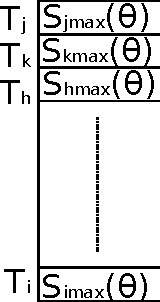
\includegraphics[scale=0.7]{figures/figure7}
\caption{\label{fig7}Values associated with $s_{max}^{*}(\theta)$}
\end{figure}


This means that the subtracted $s_{max}(\theta)$ in (\ref{eq3})
must be replaced with one of these two values ($s_{max}(\theta)$ or $\bar{s}_{max}(\theta)$). However, since we do not know  which task will interfere with $\tau_i$, the minimum is chosen, as we are determining the worst case retry cost (as this value is going to be subtracted),
and this minimum is the second maximum.

Since it is not known in priori whether $\Phi_1$ will be smaller than $\Phi_2$ for a specific $\theta$. The minimum of $\Phi_1$ and $\Phi_2$ is taken as the worst-case contribution for $\theta$ in $RC(T_i)$. Claim follows.
\end{proof}


\subsection{Upper Bound on Response Time}

To obtain an upper bound on the response time of a task $\tau_{i}$, the term $RC(T_{i})$ must be added to the workload of other tasks during the non-atomic
execution of $\tau_{i}$. But this requires modification of the WCET of each
task as follows. 
%starthere
$c_{j}$ of each interfering task $\tau_{j}$ should be inflated to accommodate for the interference of each task $\tau_{k},$ $k\ne j,i$. Meanwhile, atomic regions that access shared objects between $\tau_{j}$ and $\tau_{i}$ should not be considered in the inflation cost, because they have already been calculated in $\tau_{i}$'s retry cost. Thus, $\tau_{j}$'s inflated WCET becomes:
\begin{equation}
c_{ji}=c_{j}-\left(\sum_{\theta\in(\theta_{j}\wedge\theta_{i})}len \left(s_{j}(\theta) \right) \right)+RC(T_{ji})\label{eq9}\end{equation}
where, $c_{ji}$ is the new WCET of $\tau_{j}$ relative to $\tau_{i}$; 
the sum of lengths of all atomic sections in $\tau_{j}$ that access object $\theta$ is $\sum_{\theta \in (\theta_j \wedge \theta_i)} {len(s_{j}(\theta))}$; and $RC(T_{ji})$ is the $RC(T_j)$ 
 without including the shared objects between $\tau_{i}$ and $\tau_{j}$.
The calculated WCET is relative to task $\tau_{i}$, as it changes from task to task. The upper bound on the response time of $\tau_{i}$, denoted $R_{i}^{up}$, can be calculated iteratively, using a modification of Theorem 6 in~\cite{key-2}, as follows:
\begin{equation}
R_{i}^{up}=c_{i}+RC(T_{i})+\left\lfloor\frac{1}{m}\sum_{j\ne i}W_{ij}(R_{i}^{up})\right\rfloor
\label{eq10}
\end{equation}
where $R_{i}^{up}$'s initial value is $c_{i}+RC(T_{i})$.

$W_{ij}(R_{i}^{up})$ is calculated by (\ref{eq13}), and $W_{ij}(T_{i})$
is calculated by (\ref{eq11}), with $c_{j}$ replaced by 
$c_{ji}$, and changing~(\ref{eq12}) as:
\begin{equation}
W_{ij}(L)=max\begin{cases}
\left(\left\lceil\frac{L-\left(c_{ji}+\sum_{\theta\in(\theta_{j}\wedge\theta_{i})}len(s_{j}(\theta))\right)}{T_{j}}\right\rceil+1 \right)c_{ji}\\
\left\lceil\frac{L-c_{j}}{T_{j}}\right\rceil.c_{ji}+c_{j}-\sum_{\theta\in(\theta_{j}\wedge\theta_{i})}len(s_{j}(\theta))\end{cases}\label{eq14}\end{equation}

(\ref{eq14}) compares between two terms, as we have two cases:


\textit{Case 1}. $\tau_j^1$ (shown in Figure~\ref{fig2}) contributes by $c_{ji}$. Thus, other instances of $\tau_j$ will begin after this modified WCET, but the sum of the shared objects' atomic section lengths is removed from $c_{ji}$, causing other instances to start earlier. Thus, the term $\sum_{\theta\in(\theta_i\wedge\theta_j)} {len(s_{j}(\theta))}$ is added to $c_{ji}$ to obtain the correct start time. 

\textit{Case 2}. $\tau_j^1$ contributes by its $c_j$, but the sum of the shared atomic section lengths  between $\tau_i$ and $\tau_j$ should be subtracted from the contribution of $\tau_j^1$, as they are already included in the retry cost. 

It should be noted that subtraction of the sum of the shared objects' atomic section lengths is done in the first case to obtain the correct start time of other instances, while in the second case, this is done to get the correct contribution of $\tau_j^1$. The maximum is chosen from the two terms in (\ref{eq14}), because they differ in the contribution of their $\tau_j^1$s, and the number of instances after that.

\subsubsection{Tighter Upper Bound}

To tighten $\tau_{i}$'s response time upper bound, $RC(\tau_i)$ needs to be calculated recursively over duration $R_i^{up}$, 
and not directly over $T_i$, as done in (\ref{eq10}). So, (\ref{eq5}) must be changed to include the modified number of interfering instances. And if $R_i^{up}$ still extends to $T_i$, a situation like that shown in Figure
\ref{fig10} can happen.
\begin{figure}
\centering{}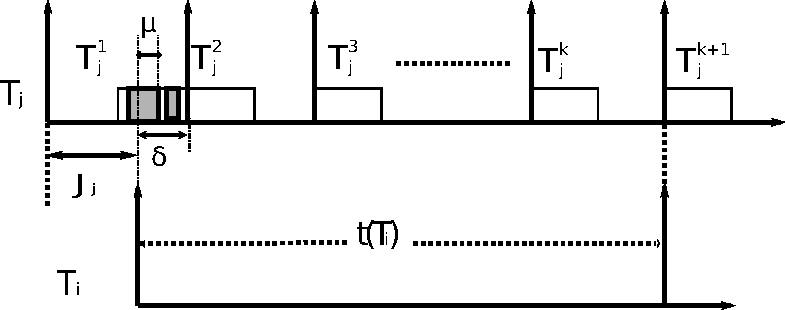
\includegraphics[scale=0.5]{figures/figure10}\caption{\label{fig10} Atomic sections of job $\tau_{j}^{1}$ contributing to period $T_i$}
\end{figure}


To counter the situation in Figure~\ref{fig10}, atomic sections of $\tau_{j}^{1}$ that are contained in the interval $\delta$
are the only ones that can contribute to $RC(T_{i})$. Of course, they can be lower, but cannot be greater, because $\tau_{j}^{1}$ has been delayed by its maximum jitter. Hence, no more atomic sections
can interfere during the duration 
$[d_j^1 -\delta,d_j^1]$.

For simplicity, we use the following notations:
\begin{compactitem}
\item $\lambda_{1}\left(j,\theta\right)=\sum_{\forall s_{j}^{l}\left(\theta\right)\in\left[d_j^1-\delta,d_j^1\right]}len\left(s_{j}^{l^{*}}\left(\theta\right)+s_{max}\left(\theta\right)\right)$
\item $\chi_{1}\left(i,j,\theta\right)=\left\lfloor\frac{T_{i}}{T_{j}}\right\rfloor\sum_{\forall s_{j}^{l}\left(\theta\right)}len\left(s_{j}^{l}\left(\theta\right)+s_{max}\left(\theta\right)\right)$
\item $\lambda_{2}\left(j,\theta\right)=\sum_{\forall s_{j}^{l}\left(\theta\right)\in\left[d_{j}^{1}-\delta,d_{j}^{1}\right]}len\left(s_{j}^{l^{*}}\left(\theta\right)+s_{max}^{*}\left(\theta\right)\right)$
\item $\chi_{2}\left(i,j,\theta\right)=\left\lfloor\frac{T_{i}}{T_{j}}\right\rfloor\sum_{\forall s_{j}^{l}\left(\theta\right)}len\left(s_{j}^{l}\left(\theta\right)+s_{max}^{*}\left(\theta\right)\right)$
\end{compactitem}
Here, $s_{j}^{l^{*}}\left(\theta\right)$ is the part of $s_{j}^{l}\left(\theta\right)$ that
is included in interval $\delta$. So, if $s_j^l (\theta)$ is partially included in $\delta$, it contributes by its included length $\mu$.

Now, (\ref{eq5}) can be modified as:
\begin{equation}
RC\left(T_{i}\right)\le \sum_{\theta\in\theta_{i}}min\begin{cases}
\begin{cases}
\Bigl(\left(\sum_{\tau_{j}\in\gamma_i\left(\theta\right)}\lambda_{1}\left(j,\theta\right)+\chi_{1}\left(i,j,\theta\right)\right)\\
-s_{max}\left(\theta\right)+s_{i_{max}}\left(\theta\right)\Bigr)\end{cases}\\
\begin{cases}
\Bigl(\left(\sum_{\tau_{j}\in\gamma_i\left(\theta\right)}\lambda_{2}\left(j,\theta\right)+\chi_{2}\left(i,j,\theta\right)\right)\\
-\bar{s}_{max}\left(\theta\right)+s_{i_{max}}\left(\theta\right)\Bigr)\end{cases}\end{cases}\label{eq15}\end{equation}



Now, to compute $RC(L)$ where $L$ does not extend to the last instance of $\tau_{j}$. Let:
\begin{compactitem}
\item $\upsilon\left(L,j\right)=\left\lceil\frac{L-c_{j}}{T_{j}}\right\rceil+1$
\item $\lambda_{3}\left(j,\theta\right)=\sum_{\forall s_{j}^{l}\left(\theta\right)}len\left(s_{j}^{l}\left(\theta\right)+s_{max}\left(\theta\right)\right)$
\item $\lambda_{4}\left(j,\theta\right)=\sum_{\forall s_{j}^{l}\left(\theta\right)}len\left(s_{j}^{l}\left(\theta\right)+s_{max}^{*}\left(\theta\right)\right)$
\end{compactitem}
Now, (\ref{eq5}) becomes: 
\begin{equation}
RC\left(L\right)\le \sum_{\theta\in\theta_{i}}min\begin{cases}
\begin{cases}
\left(\sum_{\tau_{j}\in\gamma_i\left(\theta\right)}\left(\upsilon\left(L,j\right)\lambda_{3}\left(j,\theta\right)\right)\right)\\
-s_{max}\left(\theta\right)+s_{i_{max}}\left(\theta\right)\end{cases}\\
\begin{cases}
\left(\sum_{\tau_{j}\in\gamma_i\left(\theta\right)}\left(\upsilon\left(L,j\right)\lambda_{4}\left(j,\theta\right)\right)\right)\\
-\bar{s}_{max}\left(\theta\right)+s_{i_{max}}\left(\theta\right)\end{cases}\end{cases}\label{eq16}\end{equation}


Thus, an upper bound on $RC(\tau_i)$ is given by:
\begin{equation}
RC(R_{i}^{up})\le min\begin{cases}
RC(R_{i}^{up})\\
RC(T_{i})\end{cases}
\label{eq17}
\end{equation}

Where $RC(R_i^{up})$ is calculated by~(\ref{eq16}) if $R_i^{up}$ does not extend to the last interfering instance of $\tau_j$, otherwise, it is calculated by~(\ref{eq15}). The final upper bound on $\tau_{i}$'s response time can be calculated
as in (\ref{eq10}) by replacing $RC(T_{i})$ with
$RC(R_{i}^{up})$.

\section{G-RMA/RMA CM Response Time}
\label{sec:g-rma-rma-cm}

As G-RMA is a fixed priority scheduler,  a task $\tau_{i}$ will be interfered by those tasks with priorities higher than $\tau_{i}$ (i.e., $p_{j}>p_{i}$).  Upon a conflict, the RMA CM will commit the transaction that belongs to the higher priority task. We will use \emph{RCM} to refer to a multiprocessor system scheduled by G-RMA and resolves STM conflicts by the RMA CM.


\subsection{Maximum Task Interference}


Figure~\ref{fig11} illustrates the maximum interference caused by a task $\tau_{j}$
to a task $\tau_{i}$ under G-RMA. As $\tau_{j}$ is of higher priority than $\tau_{i}$,
$\tau_{j}^{k}$ will interfere with $\tau_{i}$ even if it is not totally
included in $T_{i}$. Unlike the G-EDF case shown in Figure~\ref{fig10}, 
where only the $\delta$ part of $\tau_{j}^{1}$ is considered, in G-RMA,
$\tau_{j}^{k}$ can contribute by the whole $c_{j}$, and all atomic
sections contained in $\tau_{j}^{k}$ must be considered. This is because, in G-EDF, the worst-case pattern releases $\tau_{i}^a$ before $d_{j}^{1}$
by $\delta$ time units, and $\tau_{i}^a$ cannot be interfered before it
is released. But in G-RMA, $\tau_{i}^a$ is already released, and can be
interfered by the whole $\tau_{j}^{k}$, even if this makes it infeasible.


\begin{figure}[htbp]
\centering
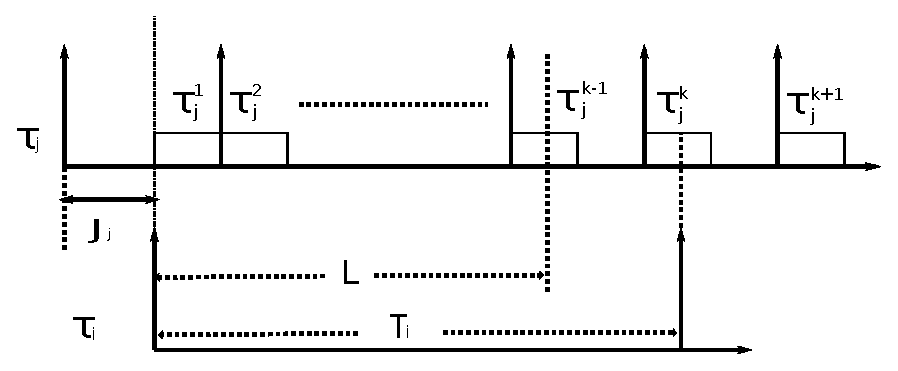
\includegraphics[scale=0.5]{figures/figure11}\caption{\label{fig11}Max interference of $T_{j}$ to $T_{i}$ in G-RMA}
\end{figure}

Thus, the maximum contribution of $\tau_{j}^b$ to $\tau_{i}^a$ for any duration
$L$ can be deduced from Figure~\ref{fig11} as $W_{ij}(L)=\left(\left\lceil\frac{L-c_{j}}{T_{j}}\right\rceil+1 \right)c_{j}$,
where $L$ can extend to $T_{i}$. In contrast to ECM where $L$ cannot be extended directly to $T_i$, as this will have a different pattern of worst case interference from other tasks.

\subsection{Retry Cost of Atomic Sections}

\begin{clm}
Under RCM, a task $\tau_i$'s retry cost over duration $L$, which can extend to $T_i$, is upper bounded by:
\begin{eqnarray}
RC\left(L\right) & \le & \sum_{\theta\in\theta_{i}}\Bigg(\left(\sum_{\tau_{j}^{*}}\left(\left(\left\lceil\frac{L-c_{j}}{T_{j}}\right\rceil+1\right)\pi\left(j,\theta\right)\right)\right)\nonumber \\
 & - & s_{max}^{min}\left(\theta\right)+s_{i_{max}}\left(\theta\right)\Bigg)\label{eq20}\end{eqnarray}
 where:
 \begin{compactitem}
\item $\tau_{j}^{*}=\{\tau_{j}|(\tau_{j}\in\gamma_i(\theta))\wedge(p_{j}> p_{i})\}$
\item $\pi(j,\theta)=\sum_{\forall s_{j}^{l}(\theta)}len\left(s_{j}^{l}\left(\theta\right)+s_{max}^{j}\left(\theta\right)\right)$
\item $s_{max}^{min}(\theta)=min_{\forall \tau_j^*} \{s_{max}^j(\theta)\}$
\end{compactitem}
\end{clm}
\begin{proof}
Since the worst case interference pattern for RCM is the same as that for ECM for an interval $L$, except that, in RCM, $L$ can extend to the entire $T_i$, but in ECM, it cannot, as the interference pattern of $\tau_j$ to $\tau_i$ changes. 
So, (\ref{eq16}) can be used to calculate $\tau_i$'s retry cost, with some modifications, as we do not have to obtain the minimum of the two terms in (\ref{eq16}), because $\tau_j$'s atomic sections will abort and retry only atomic sections of tasks with lower priority than $\tau_j$. Thus, $s_{max}(\theta)$, $s_{max}^*(\theta)$, and $\bar{s}_{max}(\theta)$ are replaced by $s_{max}^{min}(\theta)$, which is the minimum of the set of maximum-length atomic sections of tasks with priority lower than $\tau_j$ and share object $\theta$ with $\tau_i$, this is because the maximum length atomic section of tasks other than $\tau_j$ differs according to $j$. Besides, as $\tau_i$'s atomic sections can be aborted only by atomic sections of higher priority tasks, not all $\tau_j \in \gamma (\theta)$ are considered, but only the subset of tasks in $\gamma (\theta)$ with priority higher than $\tau_i$ (i.e., $\tau_j^*$). 
%Claim follows.
\end{proof}



\subsection{Upper Bound on Response Time}

The response time upper bound can be computed by Theorem 7 in~\cite{key-2} with some modification to include the effect of retry cost. Thus, this upper bound is given by:
\begin{equation}
R_{i}^{up}=c_{i}+RC(R_{i}^{up})+\left\lfloor\frac{1}{m}\sum_{j\ne i}W_{ij}(R_{i}^{up})\right\rfloor\label{eq22}\end{equation}
where $W_{ij}(R_{i}^{up})$ is calculated as in (\ref{eq14}), $c_{ji}$ is calculated by (\ref{eq9}), and $RC$ is calculated by (\ref{eq20}).

\begin{comment}
\section{FMLP and OMLP Blocking Times}
\label{sec:blocking-bound-fmlp-omlp}

The FMLP protocol~\cite{brandenburg2008comparison} has been shown to be superior to other multiprocessor real-time locking protocols in terms of schedulability, and the global OMLP protocol~\cite{key-3} has been shown to be asymptotically optimal. To formally compare STM against FMLP and global OMLP, we first upper bound their blocking times. %(those were not presented in~\cite{brandenburg2008comparison,key-4,key-3}). 


\subsection{\label{global-fmlp}Global FMLP}

FMLP can be used with global and partitioned scheduling. Since we only consider global scheduling, ``FMLP" and ``global FMLP" mean the same, for the paper's purpose.


FMLP divides shared objects into short resources, $s\_\theta$, and long ones, $l\_\theta$. Nested resources 
are grouped together into two groups: $g(s\_\theta)$ that contains only short resources, and $g(l\_\theta)$ that contains only long resources.
A request $R_i (g(s\_\theta))$ is made by a task $T_i$ to access one or more resources in $g(s\_\theta)$. This request's length is denoted $|R_i (g(s\_\theta))|$, and the number of times $T_i$ requests short resources is denoted $N_{i,s}$. Similarly, $R_i (g(l\_\theta))$ is $T_i$'s request to a group containing long resources for a duration $|R_i (g(l\_\theta))|$, and $N_{i,l}$ is the number of times $T_i$ requests long resources.


Global FMLP uses a variant of G-EDF (called GSN-EDF which discriminates between
linked jobs and scheduled ones) to account for non-preemptive jobs while still using G-EDF for scheduling, 
%%BR: "jobs"?? (can there be multiple linked jobs)?
%%BR: "ones"?? (can there be multiple scheduled ones)?
Tasks busy-wait on short resources, and suspend on long ones. In both cases, requests for resources are arranged in FIFO queues, 
%%BR: "FIFO queue" or "FIFO queues"???? (since there are two resource types)
and for requesting long resources, the task holding the resource inherits the highest priority of the suspended tasks on that resource. For short resources, there is no need to inherit priorities, as tasks become non-preemptable when acquiring short resources. 

Requests for long resources can contain requests for the short resource group, but the reverse is not true. The protocol allows non-preemptable jobs and bounds the time a job is non-preemptively blocked by a lower priority job as the maximum time a non-preemptive section of the job can be linked to the processor of the higher priority job. This non-preemptive blocking can only happen when the higher priority job is released or resumed.


Three types of blocking can be incurred by any task under global FMLP. These include busy-wait blocking, non-preemptive blocking, and direct blocking. The total blocking time of a job, $b_{i}$, is the sum of these three blocking durations. Execution time of each task, $e_{i}$, is inflated by this blocking amount ($e_{i}+b_{i}$), and is used in any of the G-EDF schedulability tests (e.g.,~\cite{Goossens:2003:PSP:876600.876615,srinivasan2002deadline}) 
for verifying schedulability. 

We upper bound a task's blocking durations due to busy-wait blocking, non-preemptive blocking, and direct blocking, denoted as $BW(T_{i})$, $NPB(T_{i})$, and $DB(T_{i})$, respectively, as follows.  
(Note that, in~\cite{key-3}, no upper bounds are presented for these terms, except for $DB(T_{i})$, as~\cite{key-3}'s main focus is on FMLP's suspension-based part. Also, the upper bound for $DB(T_{i})$ in~\cite{key-3} does not consider the effect of requesting a short resource within a long one.)


A job $T_{i}^{j}$ busy-waits in a FIFO queue when it is scheduled on a processor and it cannot be removed by any other task until its request is satisfied. As busy-waiting tasks are non-preemptable, job $T_{i}^{j}$ can be blocked for at most the maximum $m-1$ requests, where each request consists of the sum of the nested requests
to some resources in the same group. This process proceeds for each short resource requested by $T_{i}$. The busy-wait blocking time, $BW(T_{i})$, is therefore:
\begin{equation}
BW(T_{i})\le\sum_{s\_\theta\in\theta_{i}} \left(max \left[\sum_{k=1,k\ne i}^{min(m,n)-1} \left| R_{k} \left(g \left(s\_\theta \right) \right) \right| \right] \right)\label{eq26}
\end{equation}

A job $T_{i}^{j}$ can be non-preemptively blocked, either at its release or when it resumes, by at most the maximum (nested) request to any short resource. The non-preemptive blocking time, $NPB(T_{i})$, is therefore:
\begin{equation}
NPB(T_{i})=(1+N_{i,l}).max_{k\ne i} \left| R_{k}(g(s\_\theta)) \right|\label{eq27}
\end{equation}
Here, $1$ is added to $N_{i,l}$, because $T_{i}$ can be non-preemptively blocked at its release, in addition to suspension times. 

A job $T_{i}^{j}$ can be blocked by all other $n-1$ tasks for any long resource. Any of these $n-1$ requests can be a nested request to long resources belonging to the same group. In addition, any of those requests can contain a request to a short resource, and so it can busy-wait on it. Thus, each request in the $n-1$ requests, requiring access to a short resource, can be delayed by at most the maximum $m-1$ requests to the group containing that short resource. The direct blocking time, $DB(T_{i})$, is therefore:
\begin{equation}
DB(T_{i})\le\sum_{l\_\theta\in\theta_{i}} \left[max_{k=1,k\ne i}^{n-1} \left|R_{k} \left(g \left(l\_\theta \right) \right) \right| \right]
\label{eq28}
\end{equation}


\subsection{Global OMLP}


In~\cite{key-3}, 
global FMLP has a maximum s-oblivious pi-blocking cost of $\Theta(n)$, whereas global OMLP~\cite{key-3}, which is a suspension-based protocol that supports G-EDF, as well as any global job-level static priority (JLSP) scheduler, has a $\Theta(m)$ s-oblivious pi-blocking cost, as seen by equation (\ref{eq29}):
\begin{equation}
b_{i}\triangleq\sum_{k=1}^{q}N_{i,k}.2.(m-1).max_{1\le i\le n}\{L_{i,k}\}\label{eq29}\end{equation}
where $N_{i,k}$ is the maximum number of times $T_i$ requests resource $k$, and $L_{i,k}$ is the maximum execution time of such a request. $N_{i,k}$ and $L_{i,k}$ are assumed to be constants,
so the s-oblivious pi-blocking is $\Theta(m)$, and thus it is optimal.
\end{comment}

\section{STM versus Lock-Free}
\label{sec:comparison}

We now would like to understand when STM will be beneficial compared to retry-loop lock-free approach~\cite{key-5}. This retry-loop lock-free approach is the most relevant to our work. 


\subsection{\label{sub:G-EDF-scheduler-with} ECM versus Lock-Free}

\begin{clm}
For ECM's schedulability to be better or equal to that of~\cite{key-5}'s retry-loop lock-free approach,  
the size of $s_{max}$ must not exceed one half of that of $r_{max}$; with low number of conflicting tasks, the size of $s_{max}$ can be at most the size of $r_{max}$. 
\end{clm}
\begin{proof}
Equation (\ref{eq17}) can be upper bounded as:
\begin{equation}
RC\left(T_{i}\right) \le \sum_{\tau_{j}\in\gamma_{i}}\left(\sum_{\theta\in\theta_{i}}\left(\left\lceil\frac{T_{i}}{T_{j}}\right\rceil\sum_{\forall s_{j}^{l}\left(\theta\right)}\left(2.s_{max}\right)\right)\right)
\label{eq30}
\end{equation}
where $s_{j}^{l}\left(\theta\right)$, $s_{i_{max}}\left(\theta\right)$,
$s_{max}^{*}\left(\theta\right)$, and $\bar{s}_{max}\left(\theta\right)$ are replaced by $s_{max}$, and the order of the first two summations are reversed
by each other, 
with $\gamma_{i}$ being the set of tasks that share objects
with $\tau_{i}$. These changes are done to simplify the comparison.

Let $\sum_{\theta\in\theta_{i}}\sum_{\forall s_{j}^{l}\left(\theta\right)}=\beta_{i,j}^{*}$, and $\alpha_{edf}=\sum_{\tau_{j}\in\gamma_{i}}\left\lceil\frac{T_{i}}{T_{j}}\right\rceil.2\beta_{i,j}^*$. Now, (\ref{eq30}) can be modified as:
\begin{equation}
RC\left(T_{i}\right)=\alpha_{edf}.s_{max}
\label{eq31}
\end{equation}

The loop retry cost is given by:
\begin{eqnarray}
LRC\left(T_i\right)&=&\sum_{\tau_{j}\in\gamma_{i}}\left(\left\lceil\frac{T_{i}}{T_{j}}\right\rceil+1\right).\beta_{i,j}.r_{max}\nonumber \\
&=& \alpha_{free} . r_{max} \label{eq32}
\end{eqnarray}

where $\beta_{i,j}$ is the number of retry loops of $\tau_{j}$ that accesses the same object as that accessed by some retry loop of $\tau_{i}$, $\alpha_{free} = \sum_{\tau_{j}\in\gamma_{i}}\left(\left\lceil\frac{T_{i}}{T_{j}}\right\rceil + 1 \right).\beta_{i,j}$, and $r_{max}$ is the maximum execution cost of a single iteration of any retry loop of any task.
Since the shared objects are the same in both STM and lock free, $\beta_{i,j}=\beta_{i,j}^{*}$.
Thus, STM achieves equal or better schedulability 
than lock-free if the total utilization of the STM system is less than or equal to the lock-free system:
\begin{eqnarray}
\sum_{\tau_{i}}\frac{c_{i}+\alpha_{edf}.s_{max}} {T_{i}} & \le & \sum_{\tau_{i}}\frac{c_{i}+\alpha_{free}.r_{max}}{T_{i}} \nonumber \\
\therefore\frac{s_{max}}{r_{max}} & \le & \frac{\sum_{\tau_{i}}\alpha_{free}/T_{i}}{\sum_{\tau_{i}}\alpha_{edf}/T_{i}}\end{eqnarray}


Let $\bar{\alpha}_{free}=\sum_{\tau_{j}\in\gamma_{i}}\left\lceil\frac{T_{i}}{T_{j}}\right\rceil.\beta_{i,j}$,  $\hat{\alpha}_{free}=\sum_{T_{j}\in\gamma_{i}}\beta_{i,j}$, and $\alpha_{free}=\bar{\alpha}_{free}+\hat{\alpha}_{free}.$ Therefore: 
\begin{eqnarray}
\frac{s_{max}}{r_{max}} & \le & \frac{\sum_{\tau_{i}}(\bar{\alpha}_{free} +\hat{\alpha}_{free})/T_{i}}{\sum_{\tau_{i}}\alpha_{edf}/T_{i}}\nonumber \\
 & = & \frac{1}{2}+\frac{\sum_{\tau_{i}}\hat{\alpha}_{free} /T_{i}}{\sum_{\tau_{i}}\alpha_{edf}/T_{i}}
 \label{eq33}
 \end{eqnarray}

Let $\zeta_{1}=\sum_{\tau_{i}}\hat{\alpha}_{free}/T_{i}$
and $\zeta_{2}=\sum_{\tau_{i}}\left(\frac{\alpha_{edf}}{2}\right)/T_{i}$. The maximum value of $\frac{\zeta_{1}}{2.\zeta_{2}}=\frac{1}{2}$, which can happen if $T_{j}\ge T_{i}\,\therefore\left\lceil\frac{T_{i}}{T_{j}}\right\rceil=1$. Then $(\ref{eq33})=1$, which is its maximum value. $T_{j}\ge T_{i}$ means that there is small number of interferences from other tasks
to $\tau_{i}$, and thus low number of conflicts. Therefore, $s_{max}$ is
allowed to be as large as $r_{max}$.

The theoretical minimum value for $\frac{\zeta_{1}}{2.\zeta_{2}}$
is $0$, which can be asymptotically reached if $T_{j}\ll T_{i}$,
$\therefore\,\left\lceil\frac{T_{i}}{T_{j}}\right\rceil\rightarrow\infty$
and $\zeta_{2}\rightarrow\infty$. Thus, $(\ref{eq33})\rightarrow1/2$.

$\beta_{i,j}$ has little effect on $s_{max}/r_{max}$, 
as it is contained in both numerator and denominator. Irrespective of whether $\beta_{i,j}$ is going to reach its maximum or minimum value, both can be considered constants, and thus removed from (\ref{eq33})'s numerator and denominator. 
However, the number of
interferences of other tasks to $\tau_{i}$, $\left\lceil\frac{T_{i}}{T_{j}}\right\rceil$,
has the main effect on $s_{max}/r_{max}$, 
as shown in Figure~\ref{fig14}. 
\end{proof}

\begin{figure}
\begin{centering}
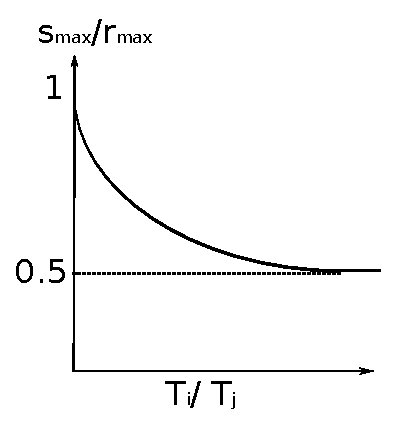
\includegraphics[scale=0.5]{figures/figure14}
\par\end{centering}
\caption{\label{fig14}Effect of $\left\lceil\frac{T_{i}}{T_{j}}\right\rceil$ on
$\frac{s_{max}}{r_{max}}$}
\end{figure}


\subsection{RCM versus Lock-Free}

\begin{clm}
For RCM's schedulability to be better or equal to that of~\cite{key-5}'s retry-loop lock-free approach, the size of $s_{max}$ must not exceed one half of that of $r_{max}$ for all cases.
However, the size of $s_{max}$ can be larger than that of $r_{max}$, depending on the number of accesses to a task $T_i$'s shared objects from other tasks.
\end{clm}
\begin{proof}
Equation (\ref{eq20}) is upper bounded by:
 \begin{equation}
\sum_{\left(\tau_{j}\in\gamma_{i}\right)\wedge\left(p_{j}> p_{i}\right)}\left(\left\lceil\frac{T_{i}-c_{j}}{T_{j}}\right\rceil+1\right).2.\beta_{i,j}.s_{max}
\label{eq34}\end{equation}

Consider the same assumptions as in Section~\ref{sub:G-EDF-scheduler-with}.
Let $\alpha_{rma}=\sum_{\left(\tau_{j}\in\gamma_{i}\right)\wedge\left(p_{j}> p_{i}\right)}\left(\left\lceil\frac{T_{i}-c_{j}}{T_{j}}\right\rceil+1\right).2.\beta_{i,j}$. Now, the ratio $s_{max}/r_{max}$ is upper bounded by:
\begin{equation}
\frac{s_{max}}{r_{max}}\le\frac{\sum_{T_{i}}\alpha_{free}/t\left(T_{i}\right)}{\sum_{T_{i}}\alpha_{rma}/t\left(T_{i}\right)}
\label{eq35}\end{equation}

The main difference between RCM and lock-free is that RCM is affected only by the higher priority tasks, while lock-free is affected by all tasks (just as in ECM). 
Besides, the RCM
is still affected by $2.\beta_{i,j}$ (just as in ECM).
The subtraction of $c_{j}$ in the numerator in (\ref{eq34}) may not
have a significant effect on the ratio of (\ref{eq35}), as the loop retry 
cost can also be modified to account for the effect of the first interfering
instance of task $T_{j}$. 
%%BR: In this paragraph, why don't you say "RCM" instead of "RMA CM"???


%%BR: Again, in the rest of this section, you can say "RCM" instead of "RMA CM"???
Therefore, 
$\alpha_{free} = \sum_{\tau_{j}\in\gamma_{i}}\left(\left\lceil\frac{T_{i}-c_j}{T_{j}}\right\rceil + 1 \right)\beta_{i,j}$.

Let tasks in the denominator of (\ref{eq35}) be given indexes $k$ instead of $i$, and $l$ instead of $j$. Let tasks in both the numerator and denominator of (\ref{eq35}) be arranged in the non-increasing priority order, so that $i=k$ and $j=l$. Let $\alpha_{free}$, in (\ref{eq35}), be divided into two parts: $\bar{\alpha}_{free}$ that contains only tasks with priority higher than $\tau_i$, and $\hat{\alpha}_{free}$ that contains only tasks with priority lower than $\tau_i$. Now, (\ref{eq35}) becomes:
\begin{eqnarray}
\frac{s_{max}}{r_{max}} & \le & \frac{\sum_{\tau_{i}}(\bar{\alpha}_{free}+\hat{\alpha}_{free})/T_{i}}{\sum_{\tau_{k}}\alpha_{rma}/T_{k}}\nonumber \\
 & = & \frac{1}{2}+\frac{\sum_{\tau_{i}}\hat{\alpha}_{free}/T_{i}}{\sum_{\tau_{k}}\alpha_{rma}/T_{k}}\label{eq36}\end{eqnarray}

For convenience, we introduce the following notations:
\begin{eqnarray}
\zeta_{1}& = & \sum_{\tau_{i}}\frac{\sum_{\left(\tau_{j}\in\gamma_{i}\right)\wedge\left(p_{j}<p_{i}\right)}\left(\left\lceil\frac{T_{i}-c_{j}}{T_{j}}\right\rceil+1\right)\beta_{i,j}}{T_{i}}\nonumber\\
& = & \sum_{T_i} \hat{\alpha}_{free}/T_i
\nonumber\\
\zeta_{2} 
& = & \sum_{\tau_{k}}\frac{\sum_{\left(\tau_{l}\in\gamma_{k}\right)\wedge\left(p_{l}>p_{k}\right)}\left(\left\lceil\frac{T_{k}-c_{l}}{T_{l}}\right\rceil+1\right)\beta_{k,l}}{T_{k}}\nonumber\\
& = & \frac{1}{2}\sum_{\tau_k} \alpha_{rma}/T_k\nonumber
\end{eqnarray}
$\tau_{j}$ is of lower priority than $\tau_{i}$, which means $D_{j}>D_{i}$. Under G-RMA, this means, $T_{j}>T_{i}$.
Thus, $\left\lceil\frac{T_{i}-c_{j}}{T_{j}}\right\rceil=1$ for
all $\tau_{j}$ and $\zeta_{1}=\sum_{\tau_{i}}(\sum_{(\tau_{j}\in\gamma_{i})\wedge(p_{j}<p_{i})}(2.\beta_{i,j}))/T_{i}$.
Since $\zeta_{1}$ contains all $\tau_{j}$ of lower priority than
$\tau_{i}$ and $\zeta_{2}$ contains all $\tau_{l}$ of higher priority than $\tau_{k}$, 
and tasks are arranged in the non-increasing priority order, then for each $\tau_{i,j}$, there exists $\tau_{k,l}$ such
that $i=l$ and $j=k$. Figure~\ref{fig:matrix-example} illustrates this, where 0 means that the pair $i,j$ 
%%BR: Whenever you say "...pair i,j,... say "...pair $(i,j)$...." The brackets help with clarity. Do this fix throughout. 
does not exist in $\zeta_{1}$,
and the pair $k,l$ does not exist in $\zeta_{2}$' (i.e., 
there is no task $\tau_l$ that is going to interfere with $\tau_k$ in $\zeta_2$), 
and 1 means the opposite. 

\begin{figure}[htbp]
\begin{tabular}{ccc}
$\begin{array}{cccccc}
 & j & 1 & 2 & \cdots & n\\
i\\
1 &  & 0 & 1 & \cdots & 1\\
2 &  & 0 & 0 & \ddots & \vdots\\
\vdots &  & \vdots & \vdots & \ddots & 1\\
n &  & 0 & 0 & \cdots & 0\end{array}$ &  & $\begin{array}{cccccc}
 & l & 1 & 2 & \cdots & n\\
k\\
1 &  & 0 & 0 & \cdots & 0\\
2 &  & 1 & 0 &  & \vdots\\
\vdots &  & \vdots & \ddots & \ddots & 0\\
n &  & 1 & \cdots & 1 & 0\end{array}$\tabularnewline
\end{tabular}
\caption{\label{fig:matrix-example} Task association for lower priority tasks than $T_i$ and higher priority tasks than $T_k$}
\end{figure}

Thus, it can be seen that both the matrices are transposes of
each other. Consequently, for each $\beta_{i,j}$, there exists $\beta_{k,l}$
such that $i=l$ and $j=k$. But the number of times $\tau_{j}$ accesses
a shared object with $\tau_{i}$ may not be the same as the number of times
$\tau_{i}$ accesses that same object. Thus, $\beta_{i,j}$ does not have
to be the same as $\beta_{k,l}$, even if $i,j$ and $k,l$ are transposes 
of each other. Therefore, we can analyze the behavior of $s_{max}/r_{max}$ based on the three parameters $\beta_{i,j}$, $\beta_{k,l}$, and $\left\lceil\frac{T_{k}-c_{l}}{T_{l}}\right\rceil$.
If $\beta_{i,j}$ is increased so that $\beta_{i,j}\rightarrow\infty$,
$\therefore\,(\ref{eq36})\rightarrow\infty$.
This is because, $\beta_{i,j}$ represents the number of times a lower priority task $\tau_{j}$ accesses 
shared objects with the higher priority task $\tau_{i}$. 
While this number has a greater effect in lock-free, it does not have any effect under RCM, because lower priority tasks do not affect higher priority
ones, so $s_{max}$ is allowed to be much greater than $r_{max}$.

Although the minimum value for $\beta_{i,j}$ is 1, mathematically, if $\beta_{i,j}\rightarrow0$, then $(\ref{eq36})\rightarrow1/2$.
Here, changing $\beta_{i,j}$ does not affect the retry cost of RCM, but it does affect the retry cost of lock-free, because the contention between tasks is reduced. Thus, $s_{max}$ is reduced in this case to
a little more than half of $r_{max}$ (``a little more''
because the minimum value of $\beta_{i,j}$ is actually 1, not 0).


The change of $s_{max}/r_{max}$ with respect to $\beta_{i,j}$ is shown in Figure~\ref{fig15-a}.
If $\beta_{k,l}\rightarrow\infty$, then (\ref{eq36})$\rightarrow1/2$.
This is because, $\beta_{k,l}$ represents the number of times
a higher priority task $\tau_{l}$ accesses shared objects with a lower
priority task $\tau_{k}$. Under RCM, this will increase the retry 
cost, thus reducing $s_{max}/r_{max}$. But if $\beta_{k,l}\rightarrow0$, then (\ref{eq36})$\rightarrow\infty$. This is due to the lower contention from a higher priority task $\tau_{l}$ to a lower priority task $\tau_{k}$, which reduces the retry cost under RCM and allows $s_{max}$ to be very large compared with $r_{max}$. Of course, the actual minimum value for $\beta_{k,l}$ is 1, and is illustrated in Figure~\ref{fig15-b}.

The third parameter that affects $s_{max}/r_{max}$ is $T_{k}/T_{l}$.
If $T_{l}\ll T_{k}$, then $\left\lceil\frac{T_{k}-c_{l}}{T_{l}}\right\rceil\rightarrow\infty$,
and $(\ref{eq36})\rightarrow1/2$. This is due to a high number
of interferences from a higher priority task $\tau_{l}$ to a lower priority
one $\tau_{k}$, which increases the retry cost under RMA CM, and consequently reduces $s_{max}/r_{max}$. 

If $T_{l}=T_{k}$ (which is
the maximum value for $T_{l}$ as $D_{l}\le D_{k}$, because
$\tau_{l}$ has a higher priority than $\tau_{k}$), then $\left\lceil\frac{T_{k}-c_{l}}{T_{l}}\right\rceil\rightarrow1$
and $\zeta_2=\sum_{\tau_{k}}\frac{\sum_{\left(\tau_{l}\in\gamma_{k}\right)\wedge\left(p_{l}>p_{k}\right)}2\beta_{k,l}}{t_{k}}$. 
This means that the system will be controlled by only two parameters, $\beta_{i,j}$, and $\beta_{k,l}$, as in the previous two cases, shown in Figures~\ref{fig15-a} and~\ref{fig15-b}. Claim follows.
\end{proof}

\begin{figure}
\begin{centering}
\subfigure[\label{fig15-a}]{\begin{centering}
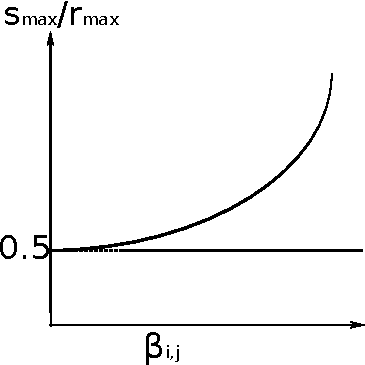
\includegraphics[scale=0.5]{figures/figure15-a}
\par\end{centering}
}\subfigure[\label{fig15-b}]{\begin{centering}
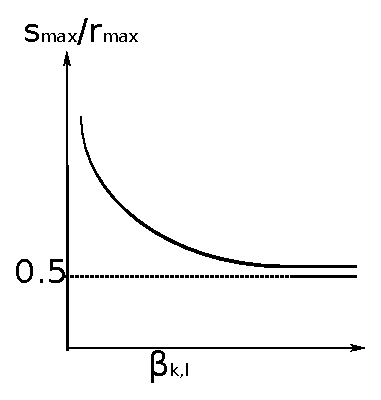
\includegraphics[scale=0.5]{figures/figure15-b}
\par\end{centering}
}
\par\end{centering}
\centering{}\caption{\label{fig15}Change of $s_{max}/r_{max}$: a) $\frac{s_{max}}{r_{max}}$
versus $\beta_{i,j}$ and b) $\frac{s_{max}}{r_{max}}$ versus $\beta_{k,l}$}
%%BR: I updated the caption, correct?
\end{figure}
\begin{comment}
\subsection{FMLP \& OMLP versus ECM and RCM
}

\begin{clm}
For ECM's schedulability to be better or equal to that of FMLP or OMLP, 
$s_{max}/|s\_\theta|_{max}$ (in case of FMLP), where $|s\_\theta|_{max}$ be the maximum short request by any task, and $s_{max}/L_{max}$ (in case of OMLP) must  not exceed $O(\frac{m}{n})$, where $L_{max}=max_{\forall i,\forall k}L_{i,k}$. For RCM's schedulability  
to be better or equal  
to that of OMLP, $s_{max}/L_{max}$ must not exceed $O(\frac{m}{n})$.
\end{clm}
\begin{proof}
As FMLP is used with G-EDF (GSN-EDF), we compare only ECM 
against it. 
%%BR: "...we compare only ECM against it."??? 
First, we derive upper bounds for the blocking parameters of FMLP. When requests are non-nested, each resource (short or long) will be contained in its own group. Let $N_{i,s}$ be the number of times a task $T_{i}$ requests a short
resource, $|s\_\theta|_{i,max}$ be the maximum request for a
short resource by $T_{i}$, $\alpha_{bw}=N_{i,s}.(m-1)$. Now, FMLP's three  blocking terms, described in Section~\ref{global-fmlp}, are upper bounded as follows:
\begin{eqnarray*}
BW(T_{i}) & \le & \sum_{s\_\theta\in\theta_{i}}(m-1).|s\_\theta|_{i,max}\\
 & = & N_{i,s}.(m-1).|s\_\theta|_{i,max}\\
 & \le & N_{i,s}.(m-1).|s\_\theta|_{max}\\
& = & \alpha_{bw}.|s\_\theta|_{max}
 \end{eqnarray*}
\begin{eqnarray*}
NPB\left(T_{i}\right) & \le & \left(1+N_{i,l}\right).max\left(BW_{k\ne i}\left(T_{k}\right)+|s\_\theta|_{k,max}\right)\\
 & \le & \left(1+N_{i,l}\right).max\left(BW_{k\ne i}\left(T_{k}\right)+|s\_\theta|_{max}\right)\\
 & = & \left(1+N_{i,l}\right).|s\_\theta|_{max}.max_{k\ne i}\left(N_{k,s}.\left(m-1\right)+1\right)\\
 & = & \alpha_{npb}.|s\_\theta|_{max}
 \end{eqnarray*}
 where $\alpha_{npb}=\left(1+N_{i,l}\right).max_{k\ne i}\left(N_{k,s}.\left(m-1\right)+1\right)$.
\begin{eqnarray*}
DB\left(T_{i}\right) & \le & N_{i,l}.\left(n-1\right).|l\_\theta|_{i,max}\\
 & \le & N_{i,l}.\left(n-1\right).|l\_\theta|_{max}\\
 \end{eqnarray*}
If $|l\_\theta|_{max}\le c1.|s\_\theta|_{max}$, where $c1$ is the
minimum constant that satisfies this relation, then
\begin{eqnarray*}
DB\left(T_{i}\right)& \le & N_{i,l}.\left(n-1\right).c1.|s\_\theta|_{max}\\
& = & \alpha_{db}.|s\_\theta|_{max}
\end{eqnarray*}
where $\alpha_{db}=N_{i,l}.\left(n-1\right).c1$. 

The total blocking time of each task is added to the task execution time, and
as before, we compare the total utilization of the G-EDF system (with both contention managers) against that under FMLP. 

Now, for ECM's schedulability to be better than FMLP,
\begin{equation}
 \frac{s_{max}}{|s\_\theta|_{max}}\le
 \frac{\sum_{T_{i}}\left(\alpha_{bw}+\alpha_{npb}+\alpha_{db}\right) \Big/t(T_{i})}{\sum_{T_{i}}\alpha_{edf} \Big/t(T_{i})}
 \label{eq38} \end{equation}

From (\ref{eq38}), it can be seen that $T_{i}$'s blocking time,
under FMLP, depends on $m,\, n$ and the number of times it requests resources
(in contrast to ECM, 
%%BR: "...contrast to ECM,..."???  
under which, $T_i$'s retry cost depends on the number of times a conflicting task $T_{j}$ requests resources). Thus, if $N_{i,s},\, N_{i,l}$, 
and $N_{k,s}$ can all be upper bounded by some constant $C_{2}$,
which is the maximum number of times any task $T_{i}$ can request a short
or long resource, then the numerator in (\ref{eq38}) 
is $O(n(n+m))$, while the denominator is $O(n^{2})$. Therefore:
\begin{equation}
\frac{s_{max}}{|s\_\theta|_{max}}=O\left(\frac{m}{n} \right)
\label{eq45}
\end{equation}
This means that, for $n<m$, the contention between tasks under both STM and
FMLP is low (even for short resources under FMLP), but FMLP is more affected
by $NTB$. When $n>m$, contention increases, but FMLP arranges
requests in a FIFO queue, so it is less affected than ECM, 
%%BR: "..than ECM,...???
which
suffers from conflicting tasks and instances
of each conflicting one. FMLP is not affected by the number of instances
of each conflicting task.

%%%%
Since OMLP's blocking time is bounded by (\ref{eq29}) \[ \therefore 
%\;
bi\le2.\left(m-1\right).L_{max}\sum_{k=1}^{q}N_{i,k}\]
%%BR: THis sentence is awkward. Why don't you say "Let  \[L_{max}=..... Since OMLP's blocking time is ..., \therefore.."


For ECM's schedulability to be better than global OMLP:
\begin{equation}
\frac{s_{max}}{L_{max}}\le\frac{\sum_{T_{i}}\left(2.\left(m-1\right)\sum_{k=1}^{q}N_{i,k}\right) \Big/t\left(T_{i}\right)}{\sum_{T_{i}}\alpha_{edf} \Big/t\left(T_{i}\right)}\label{eq40}\end{equation}

For RCM, the ratio is:
\begin{equation}
\frac{s_{max}}{L_{max}}\le\frac{\sum_{T_{i}}\left(2.\left(m-1\right)\sum_{k=1}^{q}N_{i,k}\right) \Big/t\left(T_{i}\right)}{\sum_{T_{i}}\alpha_{rma} \big/t\left(T_{i}\right)}\label{eq41}\end{equation}


If $\sum_{k=1}^{q}N_{i,k}$ is upper bounded by $C_{3}$, which is
a constant representing the maximum total number of requests for resources
by any task $T_{i}$, then:
\begin{equation}
\frac{s_{max}}{L_{max}}=O\left(\frac{nm}{n^{2}}\right)=O\left(\frac{m}{n}\right)
\label{eq46}
\end{equation}
for each of (\ref{eq40}) and (\ref{eq41}). Claim follows.
\end{proof}
\end{comment}
\section{Conclusions}
\label{sec:conclusions}

Under both ECM and RCM,  
%%BRL: "..both ECM and RCM,..." 
a task incurs $2.s_{max}$ retry cost for each of its atomic section due to a conflict with another task's atomic section. Retries under RCM and lock-free are affected by a larger number of conflicting task instances than under ECM. While task retries under ECM and lock-free are affected by all other tasks, retries under RCM are affected only by higher priority tasks. 
%%BR: Say ECM and RCM in the above paragraph, instead of EDF CM and RMA CM.


STM and lock-free have similar parameters that affect their retry costs---i.e., the number of conflicting jobs and how many times they access shared objects with a task $T_i$. The $s_{max}/r_{max}$ ratio determines whether STM is better or as good as lock-free. For ECM, this ratio cannot exceed 1, and it can be 1/2 for higher number of conflicting tasks. For RCM, for the common case, $s_{max}$ must be 1/2 of $r_{max}$, and in some cases, $s_{max}$ can be larger than $r_{max}$ by many orders of magnitude.
Our work has only further scratched the surface of real-time STM. The questions that we ask (see Section~\ref{sec:intro}) are fundamentally analytical in nature, and hence, our results are analytical. However, significant insights can be gained by experimental work on a broad range of embedded software, which is outside our work's scope. For example, what are the typical range of values for the different parameters that affect the retry cost (and hence the response time)? How tight is our retry and response time bounds in practice? Can real-time CMs be designed for other multiprocessor real-time schedulers (e.g., partitioned, semi-partitioned), and those that dynamically improve application timeliness behavior? These are important directions for further work. 


\bibliographystyle{abbrv}
\bibliography{global_bibliography}

\end{document}
